\chapter{Алгоритм оценки фазы и частоты ШПС сигнала на основе АР-модели на фоне интерференции}

\section{Применение алгоритма DMA для оценки фазы ПСП в ШПС}
\label{sec_dma_real}
Для использования параметрического метода оценки частоты необходимо восстановить гармоническую форму сигнала. Для этого
нужно получить оценку фазы ПСП и произвести повторную модуляцию входной смеси. Получить оценку фазы ПСП не прибегая к перебору по частоте,
позволяет алгоритм Delay and Multiply Approach (DMA). Данный алгоритм был представлен в статье и книге американского ученого Дж.Цуя \cite{lin_dma, tsui}.

Особенностью данного алгоритма является то, что он позволяет свести перебор в двумерной области неопределенности:
промежуточная частота, фаза ПСП к перебору только по фазе ПСП.
Пусть входная смесь представлена двумя источниками (${N=2}$. Тогда входную смесь можно записать в виде:
\begin{equation}
	\label{eq:dma_cdma_for_2}
	x(m) =	A_1 g_1(m + \tau_1) exp \left[ j \left( \tilde{\omega_1} m + \phi_1 (m) \right) \right]
		+ A_2 g_2(t + \tau_2) exp \left[ j \left(  \tilde{\omega_2} m + \phi_2 (m) \right) \right] + n(m) 
\end{equation}

Следуя алгоритму DMA, необходимо умножить входную смесь на задержанную копию:
\begin{equation}
	\label{eq:dma_cdma_1}
	xx(m) = x(m)x(m+\tau)^*,
\end{equation}
где ${*}$ - операция комплексного сопряжения, ${\tau}$ - задержка между копиями смеси. Подставляя \ref{eq:dma_cdma_for_2} в \ref{eq:dma_cdma_1} получается выражение:
\begin{eqnarray}
	\label{eq:dma_cdma_2}
	x(m) & = &[ A_1 g_1(m + \tau_1) exp \left[ j \left( \tilde{\omega_1} m + \phi_1 (m) \right) \right] + \nonumber \\
	     & + & A_2 g_2(m + \tau_2) exp \left[ j \left(  \tilde{\omega_2} m + \phi_2 (m) \right) \right] + n(m) ] + \nonumber \\
	     & + & [A_1 g_1(m + \tau + \tau_1) exp \left[ j \left( \tilde{\omega_1} (m + \tau) + \phi_1 (m + \tau) \right) \right]  + \nonumber \\
	     & + & A_2 g_2(m + \tau + \tau_2) exp \left[ j \left(  \tilde{\omega_2} (m + \tau) + \phi_2 (m + \tau) \right) \right] + n(m + \tau)]^*
\end{eqnarray}

В выражении \ref{eq:dma_cdma_2} полезным слагаемым является:
\begin{equation}
	\label{eq:dma_cdma_3}
	xx_{sig}(m) = A^2_1 g_{11}(m) exp[j (\tilde {\omega_1} \tau)],
\end{equation}
где ${g_{11}(m)}$ - новая ПСП (структура новых ПСП поясняется ниже). 

Интерференционные помехи, не содержащие полезный сигнал, могут быть представлены как:
\begin{eqnarray}
	\label{eq:dma_cdma_4}
	xx_{intf}(m) & = & A_{12} g_{12}(m) exp \left[ j \left( \tilde{\omega_1} m - \tilde{\omega_2}(m + \tau) + \phi_{12} (m) \right) \right] + \nonumber \\
		& + & A_{21} g_{12}(m) exp \left[ j \left( \tilde{\omega_2} m - \tilde{\omega_1}(m + \tau) + \phi_{21} (m) \right) \right] + \nonumber \\
		& + & A^2_2 g_{22}(m) exp[j (\tilde {\omega_2} \tau)],
\end{eqnarray}
где ${A_{12}=A_1 A_2}$, ${g_{12}(m)=g(m+\tau+1)g_2(m+\tau_2+\tau)}$, а ${g_{21} = g_2(m+\tau_2)g_1(m+\tau_1+\tau)}$, а ${g_{22}(m)}$ - новая ПСП для источника сигнала 2.

Также появляются новые шумовые компоненты:
\begin{eqnarray}
	\label{eq:dma_cdma_5}
	xx_{noise}(m) & = & A_{1} g_{1}(m + \tau_1) exp \left[ j \left( \tilde{\omega_1} m + \phi_{1} (m) \right) \right] n(m + \tau) + \nonumber \\
		& + & A_{2} g_{2}(m + \tau_2) exp \left[ j \left( \tilde{\omega_2} m + \phi_{2} (m) \right) \right] n(m + \tau)^* + \nonumber \\
		& = & n(m)A_{1} g_{1}(m + \tau_1 + \tau) exp \left[ j \left( \tilde{\omega_1} (m + \tau) + \phi_{1} (m + \tau) \right) \right] + \nonumber \\
		& + & n(m)A_{2} g_{2}(m + \tau_2 + \tau) exp \left[ j \left( \tilde{\omega_2} (m + \tau) + \phi_{2} (m + \tau) \right) \right] + \nonumber \\
		& + & n(m)n(m+\tau)
\end{eqnarray}

Таким образом \ref{eq:dma_cdma_2} можно переписать как смесь:
\begin{equation}
	\label{eq:dma_cdma_6}
	xx(m) = xx_{sig}(m) + xx_{intf}(m) + xx_{noise}(m)
\end{equation}

%%%%%%%%%%%%5
\subsection{Алгоритм DMA для одноквадратурного сигнала}
\label{sec1:dma_real}

Данный подход является достаточно интересным, но работает только с двухквадратурным приемником. Это ограничение можно
обойти, преобразуя входную смесь из действительной в комплексную, используя преобразование Гильберта.
Так же можно специальным образом выбирать ${\tau}$.

При оценке фазы ПСП в одноквадратурном приемнике возникают дополнительные сложности. Рассмотрим смесь, полученную одноквадратурным приемником:
\begin{equation}
	\label{eq:dma_real1}
	s(m) = g(m) \sin{(2\pi fm)}
\end{equation}

Задержанная версия может быть соответственно описана как:
\begin{equation}
	\label{eq:dma_real2}
	s(m - \tau) = g(m - \tau) \sin{\left[2\pi f(m-\tau)\right]}
\end{equation}

Произведение выражений \ref{eq:dma_real1} и \ref{eq:dma_real2} равно \cite{tsui}:
\begin{equation}
	\label{eq:dma_real3}
	s(m)s(m - \tau) = \frac{g(m)}{2} \left(\cos (2\pi f \tau) - \cos \left[2 \pi f (2m - \tau)\right]\right)
\end{equation}

В выражении \ref{eq:dma_real3} 2 компоненты: постоянная и высокочастотная. Высокочастотная компонента
может быть отфильтрована ФНЧ. Задержку ${\tau}$ необходимо выбирать исходя из компоненты ${\left| \cos (2\pi f \tau) \right|}$,
максимизируя значение. Нетрудно получить формулу для выбора ${\tau}$: ${\tau = \frac{1}{f} / \frac{1}{f_{samping}}}$.

\subparagraph{Недостатки}
Одним из основных недостатков является то, что данный алгоритм работает только с комплексной смесью. Модификации
для работы с действительной смесью ведут к дополнительным вычислительным затратам или потере точности. Для
преобразования Гильберта требуются дополнительные вычислительные затраты, а в формуле \ref{eq:dma_real3}, так
как ${\tau}$ заранее выбранная константа (${f\tau \approx 1}$), допплеровское смещение частоты будет снижать мощность
сигнала \ref{eq:dma_real3}, т.е.
\begin{equation}
	\left| \cos (2\pi f \tau) \right| \ge \left| \cos (2\pi (f - f_d) \tau) \right|
\end{equation}

%%%%%%%%%%%%%%%%%%%%%%%%%
\section{Алгоритм оценки параметров ШПС в условиях интерференции}
\label{l:ssec3_dma_lpc_algo}

В данной работе предлагается объединить результаты работы алгоритма DMA, рассмотренного в разделе
\ref{sec_dma_real} и, предложенных в данной работе, усовершенствованного итеративного 
алгоритма уточнения АКФ (раздел \ref{sec_acf_fft}) гармонического сигнала и 
подхода для оценки частоты ПСП-модулированного сигнала при помощи АР-модели.

Данный алгоритм был предложен автором на конференции \cite{my_dma_ar}, а так же с некоторыми доработками в \cite{my_otchet}.

Схематично алгоритм изображен на Рис. \ref{pic4:dma_quadruple_lpc}

\begin{figure}[h]
\center\scalebox{1}{\includegraphics[width=1\linewidth]{dma_quadruple_lpc.eps}}
	\caption{Алгоритм обнаружения и оценки параметров ШПС в условиях интерференции (DMA + уточненный АР)}
	\label{pic4:dma_quadruple_lpc}
\end{figure}

Выходом алгоритма DMA является оценка фазы ПСП. Повторно модулируя входную смесь с ПСП, можно восстановить гармонический сигнал. Для оценки частоты данного сигнала применяется
АР-метод. Но для оценки АР-методом, требуется точная оценка АКФ, которую можно получить
с помощью усовершенствованного итеративного алгоритма вычисления АКФ.

Рекомендации по выбору задержки ${\tau}$ и детали алгоритма DMA рассмотрены в разделе
\ref{sec1:dma_real}.

Предложенный алгоритм можно описать следующим набором шагов:
\begin{itemize}[align=left,style=nextline,leftmargin=*,labelsep=\parindent,font=\normalfont]
\item[Шаг 1.] Входная смесь ${x(k)}$ умножается на задержанную копию ${x(k-\tau)}$. Так же
	на данном шаге можно производить когерентное накопление результата, для
	увеличения ОСШ.
	\begin{equation}
		%\label{}
		x_{new}(k) = \frac{g_{new}(k)}{2} \left(\cos (2\pi f \tau) - \cos \left[2 \pi f (2t - \tau)\right]\right)
	\end{equation}

\item[Шаг 2.] Полученная смесь ${x_{new}(k)}$ фильтруется ФВЧ для отсечения высокочастотной компоненты.
\item[Шаг 3.] Генерируется локальная ПСП ${g(k)}$ и умножается на задержанную копию ${g(k-\tau)}$.
	\begin{equation}
		%\label{}
		g_{new}(k) = g(k)g(k-\tau)
	\end{equation}

\item[Шаг 4.] Отфильтрованная смесь ${x_{filt}(k)}$ коррелируется с новой ПСП ${g_{new}(k)}$
	с использованием БПФ. Выход коррелятора сравнивается с заранее определенным порогом.
	\begin{equation}
		%\label{}
		x_{filt}(k) = \frac{g_{new}(k)}{2} \cos (2\pi f \tau)
	\end{equation}

	\subitem{\bf{Если}}  значение оказалось больше порогового {\bf{то}},
		принимается решение о наличии сигнала. Полученное значение фазы ПСП  - ${m}$ запоминается.
		Перейти на шаг 5.
	\subitem{\bf{Иначе}} 
		Принимается решение об отсутствии сигнала.
\item[Шаг 5.] Входная смесь ${x(k)}$ модулируется ПСП ${g(k-m)}$. В результате получаем смесь с гармонической компонентой 
	${x_{cos}(k)}$ с неизвестной частотой.
\item[Шаг 6.] Для увеличения ОСШ сигнала ${x_{cos}(k)}$ вычисляется значение уточненное значение АКФ
	по алгоритму, предложенному в разделе \ref{l:sec_acf}.
\item[Шаг 7.] Определяются коэффициенты АР-модели ${\hat{a_1}, \hat{a_2}}$, по формуле \ref{eq:lpc_a_estimation}. 
	Вычисляется резонансная частота ${\omega_0 = 2 \pi f}$ и определяется квадрат модуля частотного отклика АР-модели для этой частоты. 
\end{itemize}

Количество умножений требуемых для оценки частоты одного источника при помощи алгоритма Delay and Multiply Approach и АР-модели:
\begin{enumerate}
\item Алгоритм DMA:
	\begin{equation}
		%\label{}
		OP_{DMA} = 8NlogN + 6N
	\end{equation}
\item Усовершенствованный итеративный алгоритм получения АКФ:
	\begin{equation}
		%\label{}
		OP_{ACF} = 8NlogN + (k+2)N
	\end{equation}
\item Оценка параметра АР-методом:
	\subitem Обращение АКФ матрицы 2x2 элементов требует: 5 умножений, 1 обращение и 1 сложение;
	\subitem Вычисление параметров АР-модели: 4 умножения, 2 сложения;
	\subitem Вычисление полюсов передаточной функции АР-модели: 2 умножения, 3 сложения, 1 операция извлечения корня.
	\begin{equation}
		%\label{}
		OP_{AR} = 51
	\end{equation}
\end{enumerate}

Следует отметить, что в пункте 3 произведены допущения: стоимость 1 операции деления равна 10 операциям умножения, стоимость операции извлечения
корня составляет 20 операций умножения, стоимость сложения не учитывается.
Общее количество умножений для оценки частоты при помощи развиваемого подхода при учете трех итераций уточнения АКФ:
\begin{equation}
	%\label{}
	OP_{DMA\_ACF\_AR} = 16NlogN + 11N
\end{equation}

%%%%%%%%%%%%%%
\section{Сравнительный анализ с параллельным коррелятором}
Структура программного приемника СПИ  Navstar GPS рассмотрена в \cite{tsui}. После стадии оценки параметров сигнала и сравнения с порогом, оценка
частоты для заданного источника поступает в модуль уточнения частоты. Уточненная частота и фаза ПСП поступают в ФАПЧ.
Одним из параметров системы ФАПЧ является шумовая полоса. Этот параметр определяет количество теплового шума попадающего в систему ФАПЧ.
Широкая шумовая полоса позволяет системе ФАПЧ быстро войти в синхронизм, но также ведет к существенному ухудшению характеристик системы ФАПЧ за счет возрастания уровня теплового шума. 

Область синхронизации частоты, в пределах которой не обеспечивается срыв синхронизации, определяется как \cite{spilker-book}:
\begin{equation}
	\label{eq:pll_omega_m}
	\Delta \omega_m \approx 2 \omega_n (\zeta+0.6),
\end{equation}
где ${\omega_n}$ - собственная частота системы ФАПЧ, ${\zeta}$ - коэффициент демпфирования(${\zeta > 0.3}$).

Примем ${\zeta = 0.707}$. Данное значение   близко к оптимальному \cite{tsui, spilker-book}, тогда ${\Delta \omega_m = 2.614 \omega_n}$.
Собственная частота системы ФАПЧ вычисляется по формуле:
\begin{equation}
	\label{eq:pll_omega_n}
	\omega_n = \frac{8 \zeta B_L}{4 \zeta^2 + 1},
\end{equation}
где ${B_L}$ - шумовая полоса.

Традиционный подход к оценке параметров широкополосного сигнала предусматривает корреляцию входной смеси и набора локальных копий сигнала шагом 1 кГц.
Для стационарного приемника СПИ Navstar GPS диапазон смещения частоты, обусловленный Доплеровским эффектом, находится в диапазоне ${\pm 5}$ кГц \cite{tsui, shahtarin_sync}.
Таким образом, для получения оценки с точностью 1 кГц необходимо провести поиск в 11 ячейках. В каждой ячейке нам необходимо ${N}$-комплексных умножений.
Для наземных приемников типовое значение ${B_L=20}$ Гц \cite{tsui}. Область синхронизации из выражений \ref{eq:pll_omega_m} и \ref{eq:pll_omega_n}
${\Delta \omega_m = 100}$ рад/с. В виду того, что требуемая точность оценки не может быть получена с использованием стандартного шага в 1 кГц,
а использование более мелкого шага ведет к расходованию ресурсов, как уже было отмечено, требуется стадия уточнения частоты.
Схема традиционного приемника изображена на Рис. \ref{pic:corr_scheme}.
\begin{figure}[h]
	\center\scalebox{1}{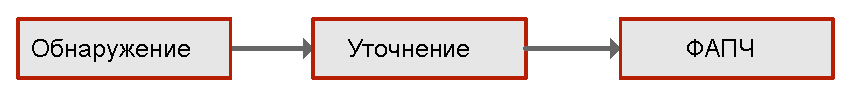
\includegraphics[width=1\linewidth]{corr_scheme.eps}}
	\caption{Схема традиционного приемника.}
	\label{pic:corr_scheme}
\end{figure}

Количество комплексных умножений требуемых для оценки частоты одного источника при помощи алгоритма БПФ:
\begin{enumerate}
\item ${NlogN}$ - преобразование Фурье входной смеси;
\item ${N}$ - умножение входного смеси и локальной копии сигнала в Фурье домене;
\item ${N}$ - обратное преобразование Фурье.
\item ${4NlogN}$ - действительных умножений – обратное преобразование Фурье. 
\end{enumerate}
\begin{equation}
	\label{eq:op_fft}
	OP_{FFT} = NlogN + 11(N + NlogN) = 12NlogN + 11N
\end{equation}

Алгоритм уточнения частоты описан в \cite{tsui}. Данный алгоритм основан на усреднении фазы и требует дополнительной оперативной памяти (ОЗУ) приемника для
хранения 5 миллисекунд данных при обработке одного источника. Оперативная память потребляет значительное количество энергии, поэтому снижение количества
необходимой ОЗУ является важной задачей при разработке портативных приемников. Также обработка 5 мс данных повышает вероятность встретить переход бита
внутри данных – это ведет к дополнительным сложностям при реализации программных приемников сигнала Navstar GPS.

Количество умножений, требуемых для уточнения частоты одного источника:
\begin{enumerate}
\item Повторная модуляция 5 мс данных: ${5N}$ умножений;
\item Повышение точности до 400 Гц: ${6N}$ умножений;
\item Вычисление ДПФ в частотной позиции на длине: ${10N}$ умножений.
\end{enumerate}
\begin{equation}
	\label{eq:op_fine}
	OP_{FINE} = 21N
\end{equation}

Общее количество операций умножения (количество операций комплексного умножения необходимо домножить на 4):  .
\begin{equation}
	\label{eq:op_fine_fft}
	OP_{FFT\_FINE} = 48NlogN + 65N
\end{equation}

%%%%%%%%%%%%%%%%
\section{Сравнение точности оценки частоты с границей Крамера-Рао}
При разработке алгоритмов оценки параметров полезно иметь некоторую базу для сравнения. Такой базой может быть выбрана граница Крамера-Рао.

Оценка Крамера-Рао тесно связана с понятием эффективности . Данная граница эффективности оценки, улучшить которую невозможно, описывается
неравенством Крамера-Рао-Фреше. Так же известное как неравенство информации.

Если рассматривать класс всевозможных оценок ${\hat{\theta}}$ оцениваемого скалярного параметра ${\theta}$, от которого зависит ПРВ ${f(X; \theta)}$
исследуемой совокупности. Обозначим
\begin{equation}
	\label{eq:clrb_mean}
	{\bf{E}} \hat{\theta} = \int \hat{\theta} (X_1, ..., X_n)L(X_1, ..., X_n; \theta) dX_1 ... dX_n= \theta + b_{\hat{\theta}}(\theta),
\end{equation}
${b_{\hat{\theta}}(\theta)}$ дает смещение оценки ${\theta}$.

В \cite{ayvazyan-book} приведено, что если  ПРВ ${f(X, \theta)}$  
удовлетворяет некоторым  условиям регулярности (в смысле характера ее зависимости от ${\theta}$), а именно:
\begin{enumerate}
\item область возможных значений исследуемой случайной величины в которой ${f(X; \theta)}$, не зависит от ${\theta}$;
\item в формуле \ref{eq:clrb_mean} и в тождестве ${\int L(X_1, ..., X_n;\theta) dX_1...dX_n = 1}$ допустимо дифференцирование по ${\theta}$ под знаком интеграла;
\item величина ${I(\theta; X)}$ - количество информации Фишера не равна нулю.
\end{enumerate}

Тогда для любой оценки ${\hat{\theta}}$ оцениваемого параметра ${\theta}$ может быть записано неравенство:
\begin{equation}
	\label{eq:crlb_base3}
	E(\hat{\theta} - \theta) \ge \frac{(1 + \frac{d b_{\hat{\theta}} (\theta)}{d \theta})^2}{n E \left[ \left( \frac{d ln f(X; \theta)}{d \theta} \right)^2 \right]}
\end{equation}

\subsection{Граница Крамера-Рао для оценки одной гармонической компоненты}
В данной работе рассматривается оценка частоты одной гармонической компоненты. Поэтому целесообразно рассмотреть только данный случай. В статье \cite{rife-crlb-article}
подробно рассмотрено получение оценки Крамера-Рао для случае одной гармонической компоненты, далее приводится краткая сводка результатов.

Предположим один или несколько параметров сигнала неизвестны. Входная смесь представлена синфазной и квадратурной составляющими. Тогда совместная ПРВ ${\bf{X}}$
при векторе неизвестных параметров ${\bf{\alpha}}$  может быть записана как:
\begin{equation}
	\label{eq:clrb_pdf}
	f({\bf{X}}; {\bf{\alpha}}) = \left( \frac{1}{\sigma^2 2 \pi} \right)^N exp \left[ -\frac{1}{2\sigma^2} \sum_{n=0}^{N-1} (Re(x)-\mu_n)^2 + (Im(x) - \nu_n)^2 \right],
\end{equation}
где
\begin{eqnarray}
	\label{eq:clrb_alpha}
	{\bf{\alpha}} & = & [\omega, A, \theta]^T \\
	\mu_n & = & A \cos{(\omega t + \theta)} \\
	\nu_n & = & A \sin{(\omega t + \theta)}
\end{eqnarray}

Несмещенная оценка Крамера-Рао состоит из диагональных элементов матрицы обратной к информационной матрице Фишера ${J}$, таких что
\begin{equation}
	\label{eq:crlb_Jij}
	J_{ij} = E(H_{\alpha i} H_{\alpha j}) = -E(H_{\alpha i \alpha j}),
\end{equation}
где математическое ожидание с учетом вектора ${\bf{X}}$:
\begin{equation}
	\label{eq:crlb_H}
	H_{\alpha i} = \frac{\partial}{\partial \alpha_i} \log{f({\bf{X}}; {\bf{\alpha}})}
\end{equation}
Граница задается как:
\begin{equation}
	\label{eq:crlb_var_alpha}
	D(\hat{\alpha}_i) \ge J^{ii},
\end{equation}
где ${\hat{\alpha}}$ - это оцениваемый параметр ${\alpha_i}$ и ${J^{ii}}$ - ${i}$-й диагональный элемент матрицы ${J^{-1}}$.

Когда ${f({\bf{X}}; {\bf{\alpha}})}$ задана выражением \ref{eq:clrb_pdf}, элементы матрицы ${J}$ могут быть получены с использованием следующего соотношения:
\begin{equation}
	\label{eq:crlb_Jij_full}
	J_{ij} = \frac{1}{\sigma^2} \sum_{n=0}^{N-1} \left[ \frac{\partial \mu_n}{\partial \alpha_i} \frac{\partial \mu_n}{\partial \alpha_j} + \frac{\partial \nu_n}{\partial \alpha_i} \frac{\partial \nu_n}{\partial \alpha_j} \right]
\end{equation}
Индексы ${i}$ и ${j}$ относятся только к неизвестным параметрам ${\alpha}$.

Наиболее общим случаем для всех параметров ${\alpha}$, матрица ${J}$ из \ref{eq:crlb_Jij_full} принимает вид:
\begin{equation}
	\label{eq:lpc_a_estimation}
	J = \frac{1}{\sigma^2} =
		\left[ \begin{array}{ccc}
			A_0^2 T^2 (n_0^2 N + 2n_0P + Q) & 0 & A_0^2 T^2 (n_0 N + P) \\
			0 & N & 0 \\
			A_0^2 T^2 (n_0 N + P) & 0 & A_0^2N
		\end{array} \right]
\end{equation}
где
\begin{eqnarray}
	\label{eq:clrb_QP}
	P & = & \sum_{n=0}^{N-1}n = \frac{N(N-1)}{2} \\
	Q & = & \sum_{n=0}^{N-1}n^2 = \frac{N(N-1)(2N-1)}{6}
\end{eqnarray}

Матрица ${J}$ может быть получена из \ref{eq:crlb_Jij_full} для всех возможных комбинаций. В случае если фаза известна матрица ${J}$ становится матрицей 2x2, после удаления третьей строки
и третьего столбца.

После получения обратной матрицы ${J}$, с учетом всех неизвестных параметров, можно получить следующие выражения.
Для известной фазы и известной или неизвестной амплитуды:
\begin{equation}
	\label{eq:clrb_est_omega_1}
	D(\hat{\omega}) \ge \frac{\sigma^2}{A_0^2 T^2 (n_0^2 N + 2n_0P + Q)}
\end{equation}

Для неизвестной фазы и известной или неизвестной амплитуды:
\begin{equation}
	\label{eq:clrb_est_omega_2}
	D(\hat{\omega}) \ge \frac{12\sigma^2}{A_0^2 T^2N(N^2-1)}
\end{equation}

Для всех случаев:
\begin{equation}
	\label{eq:clrb_est_b_1}
	D(\hat{A}) \ge \frac{\sigma^2}{N}
\end{equation}

Для известной частоты и известной или неизвестной амплитуды:
\begin{equation}
	\label{eq:clrb_est_b_1}
	D(\hat{\theta}) \ge \frac{\sigma^2}{A_0^2N}
\end{equation}

Для неизвестной частоты и известной или неизвестной амплитуды:
\begin{equation}
	\label{eq:clrb_est_b_1}
	D(\hat{\theta}) \ge \frac{12\sigma^2(n_0N + 2n_0P + Q)}{A_0^2N(N^2-1)}
\end{equation}

\section{Сравнение предлагаемого алгоритма с границей Крамера-Рао}
\begin{figure}[h]
\center\scalebox{1}{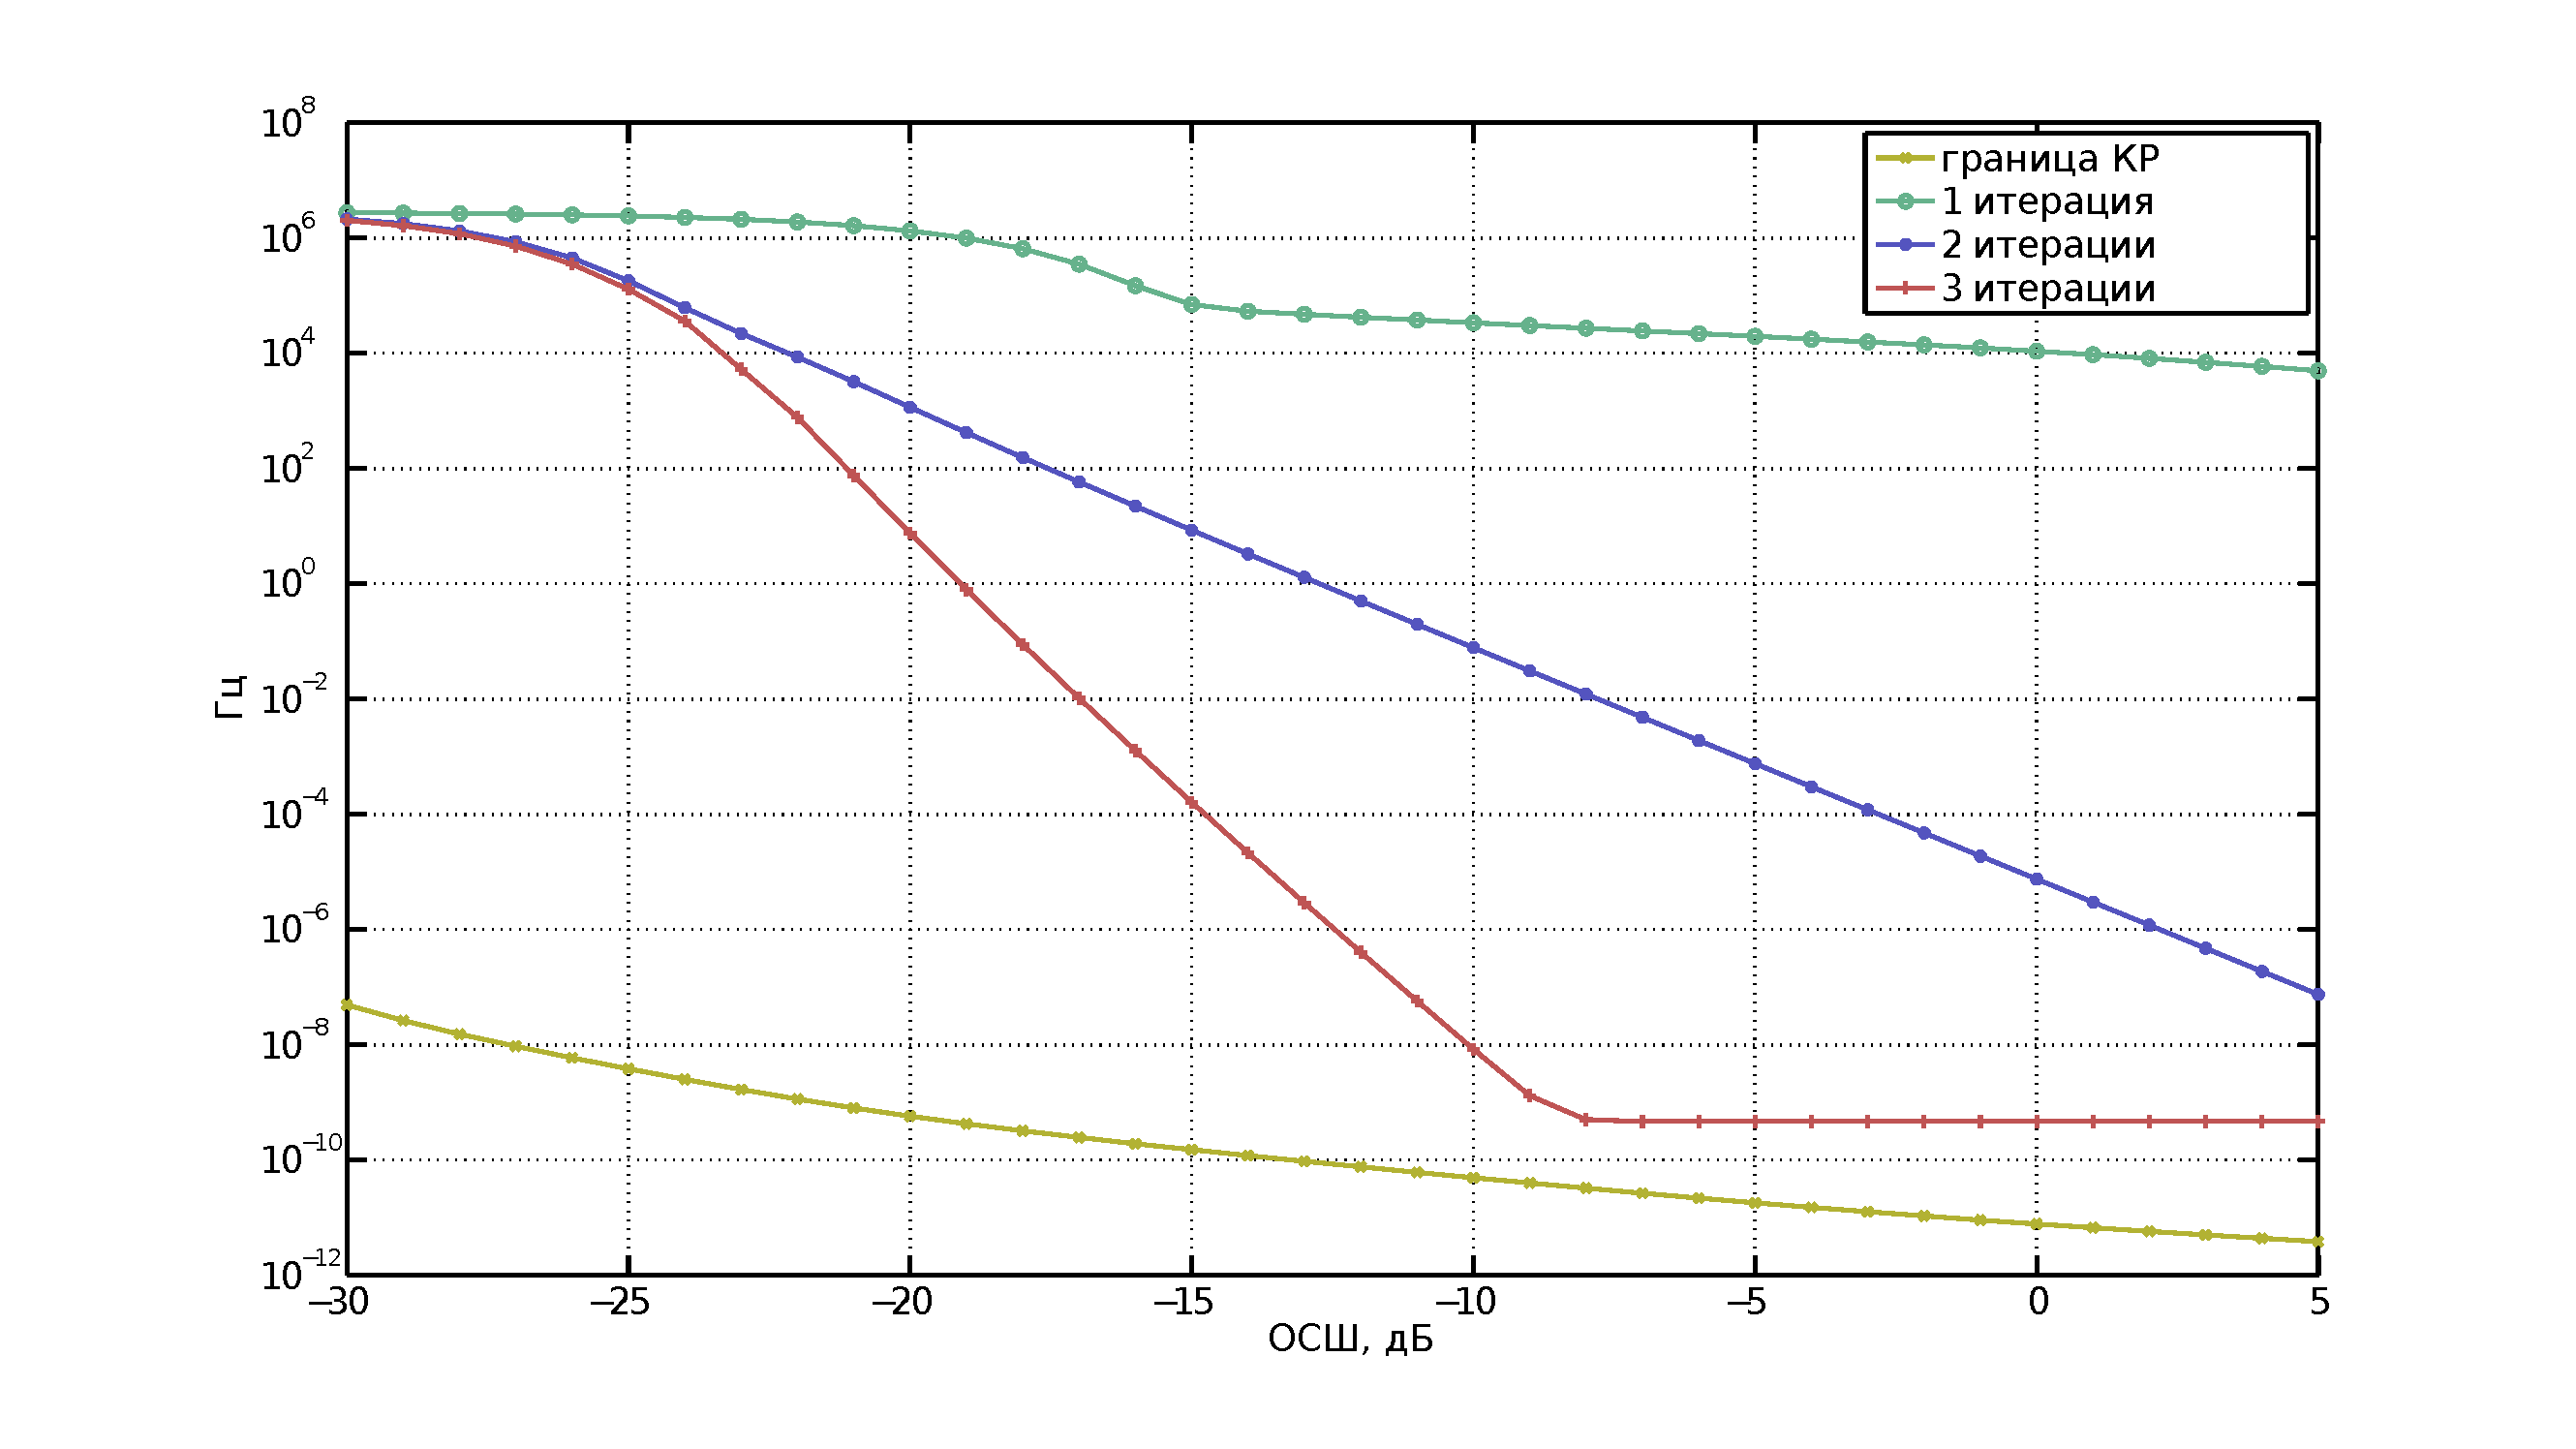
\includegraphics[width=1\linewidth]{crlb_vs_algorithm.eps}}
	\caption{СКО оценки частоты при использовании итеративного алгоритма оценки АКФ и АР модели}
	\label{pic:crlb_vs_algorithm}
\end{figure}

Из Рис. \ref{pic:crlb_vs_algorithm} видно, что используя итеративный алгоритм вычисления АКФ можно получить заданную точность
при ОСШ -13 дБ для 2 итераций и -20 дБ для 3 итераций. Моделирование проводилось на частоте кратной частоте дискретизации для
того чтобы избежать эффектов растекания спектра. Данные эффекты можно частично компенсировать дополнением нулями в
усовершенствованном итеративном алгоритме получения АКФ. Это было учтено при полунатурном моделировании.

\section{Выводы}
%В данном случае необходима стадия уточнения частоты. Следует отметить, что заданная точность может быть достигнута даже на сигнале с достаточно
%низким ОСШ при оценке АР-методом после уточнения АКФ – .рисунок 8.

В данной главе рассмотрен метод оценки параметров ШПС. Проведено сравнение с существующим методом оценки параметров СПИ с ШПС. На основании рассмотренного материала можно заключить:
\begin{enumerate}
\item Особенностью СПИ с ШПС является наличие ярко выраженного одиночного пика на ПЧ в спектральной области после повторной модуляции смеси с ПСП.
	Этот факт дает основания полагать, что такие сигналы могут быть достаточно точно представлены с помощью АР(2) модели.
\item Использование процедуры оценки параметров АР(2) вместо перебора по заранее заданным значениям позволяет вести поиск сигнала в широком диапазоне частот и определять сдвиг
	с более высокой точностью, устраняя необходимость дополнительного уточнения доплеровского сдвига перед запуском процедуры сопровождения сигнала.
\item Точность оценок, полученных на основе АР(2) быстро снижается при наличии сильного или окрашенного шума. Для преодоления указанных трудностей в 
	данной работе предлагается использовать усовершенствованный итеративный алгоритм уточнения АКФ (глава \ref{sec_acf_fft}).
\item Вычислительные затраты предложенного алгоритма составляют   операций умножения, что значительно ниже чем   для традиционного алгоритма параллельного коррелятора.
\end{enumerate}

Сказанное выше позволяет заключить, что разработанный алгоритм может применяться в задачах оценки параметров СПИ с ШПС в случаях когда размер выборки ограничен и
требуется повышенная точность оценки доплеровского сдвига частоты. К недостаткам метода следует отнести высокие требования к точности выполнения математических операций.
Так, например, при вычислении полюсов передаточной функции АР модели необходимо использовать вычисления в формате с плавающей точкой. 
Как уже было сказано, моделирование проводилось на частоте, кратной частоте дискретизации. Данное ограничение можно преодолеть используя дополнение нулями при оценке АКФ
в усовершенствованном алгоритме оценки АКФ.

\subsection{Выводы по Главе 3}

\begin{itemize}
\item Алгоритм, предложенный в работе, может быть реализован на современной аппаратной платформе в виде программного приемника (SDR). 
\item Точность оценки, полученная на выходе предлагаемого алгоритма, позволяет без дополнительной стадии оценки частоты запустить модуль ФАПЧ.
\item Алгоритм может быть использован при работе в реальных приемниках.
\end{itemize}

\clearpage
